\documentclass[a4paper]{report}
\usepackage[utf8]{inputenc}
\usepackage[T1]{fontenc}
\usepackage{RJournal}
\usepackage{amsmath,amssymb,array}
\usepackage{booktabs}


% tightlist command for lists without linebreak
\providecommand{\tightlist}{%
  \setlength{\itemsep}{0pt}\setlength{\parskip}{0pt}}

\usepackage{longtable}

% Always define CSL refs as bib entries are contained in separate doc
% Pandoc citation processing
%From Pandoc 3.1.8
% definitions for citeproc citations
\NewDocumentCommand\citeproctext{}{}
\NewDocumentCommand\citeproc{mm}{%
  \begingroup\def\citeproctext{#2}\cite{#1}\endgroup}
\makeatletter
 % allow citations to break across lines
 \let\@cite@ofmt\@firstofone
 % avoid brackets around text for \cite:
 \def\@biblabel#1{}
 \def\@cite#1#2{{#1\if@tempswa , #2\fi}}
\makeatother
\newlength{\cslhangindent}
\setlength{\cslhangindent}{1.5em}
\newlength{\csllabelwidth}
\setlength{\csllabelwidth}{3em}
\newenvironment{CSLReferences}[2] % #1 hanging-indent, #2 entry-spacing
 {\begin{list}{}{%
  \setlength{\itemindent}{0pt}
  \setlength{\leftmargin}{0pt}
  \setlength{\parsep}{0pt}
  % turn on hanging indent if param 1 is 1
  \ifodd #1
   \setlength{\leftmargin}{\cslhangindent}
   \setlength{\itemindent}{-1\cslhangindent}
  \fi
  % set entry spacing
  \setlength{\itemsep}{#2\baselineskip}}}
 {\end{list}}
\usepackage{calc}
\newcommand{\CSLBlock}[1]{#1\hfill\break}
\newcommand{\CSLLeftMargin}[1]{\parbox[t]{\csllabelwidth}{#1}}
\newcommand{\CSLRightInline}[1]{\parbox[t]{\linewidth - \csllabelwidth}{#1}\break}
\newcommand{\CSLIndent}[1]{\hspace{\cslhangindent}#1}


\usepackage{float, longtable}

\begin{document}


%% do not edit, for illustration only
\sectionhead{Contributed research article}
\volume{17}
\volnumber{1}
\year{2025}
\month{March}

\begin{article}
  % !TeX root = RJwrapper.tex
\title{Changes on CRAN}

\subtitle{%
2025-01-01 to 2025-03-31
}

\author{by Kurt Hornik, Uwe Ligges, and Achim Zeileis}

\maketitle


\section{CRAN growth}\label{cran-growth}

In the past 3 months, 528~new packages were
added to the CRAN package repository. 142~packages
were unarchived, 274~were archived and
0~had to be removed. The following shows the
growth of the number of active packages in the CRAN package repository:

\begin{center}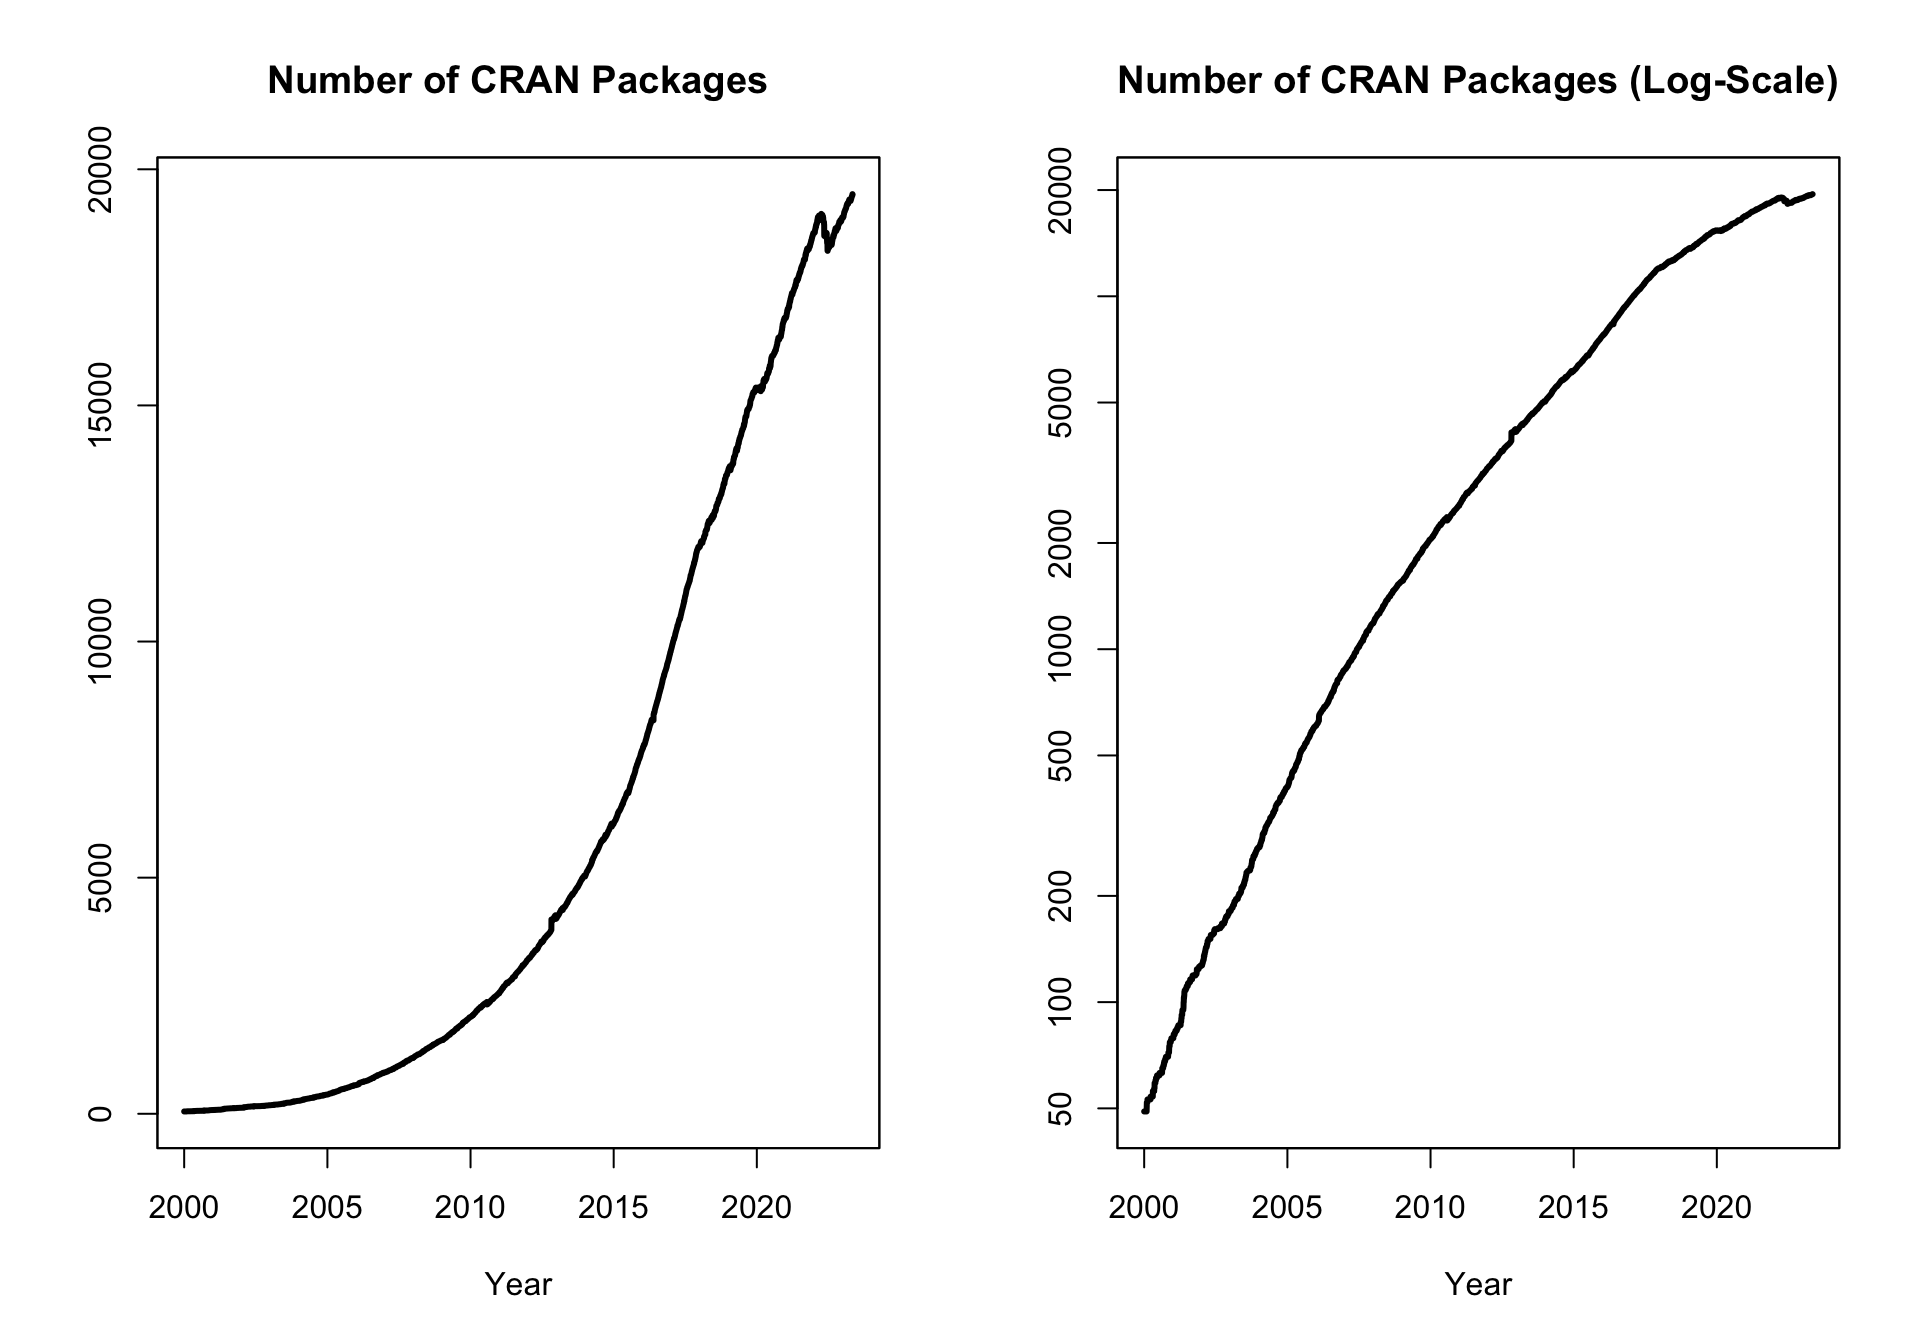
\includegraphics[width=1\linewidth,alt={CRAN growth: Number of CRAN packages over time in levels (left) and in logs (right).}]{RJ-2025-1-cran_files/figure-latex/cran_growth-1} \end{center}

\noindent On 2025-03-31, the number of active packages was around~22253.

\section{CRAN package submissions}\label{cran-package-submissions}

From January 2025 to March 2025
CRAN received 7690~package submissions.
For these, 12213~actions took place of which
9271~(76\%) were auto processed actions and
2942~(24\%) manual actions.

Minus some special cases, a summary of the auto-processed and manually
triggered actions follows:

\begin{longtable}[]{@{}
  >{\raggedright\arraybackslash}p{(\linewidth - 16\tabcolsep) * \real{0.0986}}
  >{\raggedleft\arraybackslash}p{(\linewidth - 16\tabcolsep) * \real{0.1127}}
  >{\raggedleft\arraybackslash}p{(\linewidth - 16\tabcolsep) * \real{0.1127}}
  >{\raggedleft\arraybackslash}p{(\linewidth - 16\tabcolsep) * \real{0.1127}}
  >{\raggedleft\arraybackslash}p{(\linewidth - 16\tabcolsep) * \real{0.1127}}
  >{\raggedleft\arraybackslash}p{(\linewidth - 16\tabcolsep) * \real{0.1127}}
  >{\raggedleft\arraybackslash}p{(\linewidth - 16\tabcolsep) * \real{0.1127}}
  >{\raggedleft\arraybackslash}p{(\linewidth - 16\tabcolsep) * \real{0.1127}}
  >{\raggedleft\arraybackslash}p{(\linewidth - 16\tabcolsep) * \real{0.1127}}@{}}
\toprule\noalign{}
\begin{minipage}[b]{\linewidth}\raggedright
\end{minipage} & \begin{minipage}[b]{\linewidth}\raggedleft
archive
\end{minipage} & \begin{minipage}[b]{\linewidth}\raggedleft
inspect
\end{minipage} & \begin{minipage}[b]{\linewidth}\raggedleft
newbies
\end{minipage} & \begin{minipage}[b]{\linewidth}\raggedleft
pending
\end{minipage} & \begin{minipage}[b]{\linewidth}\raggedleft
pretest
\end{minipage} & \begin{minipage}[b]{\linewidth}\raggedleft
publish
\end{minipage} & \begin{minipage}[b]{\linewidth}\raggedleft
recheck
\end{minipage} & \begin{minipage}[b]{\linewidth}\raggedleft
waiting
\end{minipage} \\
\midrule\noalign{}
\endhead
\bottomrule\noalign{}
\endlastfoot
auto & 2798 & 623 & 1622 & 152 & 0 & 2401 & 931 & 356 \\
manual & 1171 & 4 & 13 & 6 & 60 & 1307 & 276 & 98 \\
\end{longtable}

These include the final decisions for the submissions which were

\begin{longtable}[]{@{}lrr@{}}
\toprule\noalign{}
& archive & publish \\
\midrule\noalign{}
\endhead
\bottomrule\noalign{}
\endlastfoot
auto & 2672 (35.5\%) & 2179 (28.9\%) \\
manual & 1157 (15.4\%) & 1522 (20.2\%) \\
\end{longtable}

\noindent where we only count those as \emph{auto} processed whose publication or
rejection happened automatically in all steps.

\section{CRAN mirror security}\label{cran-mirror-security}

Currently, there are 93 official CRAN mirrors,
77~of which provide both
secure downloads via `\texttt{https}' \emph{and} use secure mirroring from the CRAN master
(via rsync through ssh tunnels). Since the~R 3.4.0 release, \texttt{chooseCRANmirror()}
offers these mirrors in preference to the others which are not fully secured (yet).

\section{CRAN Task View Initiative}\label{cran-task-view-initiative}

There are two new task views:

\begin{itemize}
\tightlist
\item
  \href{https://CRAN.R-project.org/view=CompositionalData}{Compositional Data Analysis}: Maintained by Karel Hron, Javier Palarea-Albaladejo, Matthias Templ, Alessandra Menafoglio.
\item
  \href{https://CRAN.R-project.org/view=NetworkAnalysis}{Network Analysis}: Maintained by Fabio Ashtar Telarico, Pavel N. Krivitsky, James Hollway.
\end{itemize}

Currently there are 48~task views (see \url{https://CRAN.R-project.org/web/views/}),
with median and mean numbers of CRAN packages covered
108 and~122, respectively.
Overall, these task views cover 4906~CRAN packages,
which is about 22\% of all active CRAN packages.


\address{%
Kurt Hornik\\
WU Wirtschaftsuniversität Wien\\%
Austria\\
%
%
\textit{ORCiD: \href{https://orcid.org/0000-0003-4198-9911}{0000-0003-4198-9911}}\\%
\href{mailto:Kurt.Hornik@R-project.org}{\nolinkurl{Kurt.Hornik@R-project.org}}%
}

\address{%
Uwe Ligges\\
TU Dortmund\\%
Germany\\
%
%
\textit{ORCiD: \href{https://orcid.org/0000-0001-5875-6167}{0000-0001-5875-6167}}\\%
\href{mailto:Uwe.Ligges@R-project.org}{\nolinkurl{Uwe.Ligges@R-project.org}}%
}

\address{%
Achim Zeileis\\
Universität Innsbruck\\%
Austria\\
%
%
\textit{ORCiD: \href{https://orcid.org/0000-0003-0918-3766}{0000-0003-0918-3766}}\\%
\href{mailto:Achim.Zeileis@R-project.org}{\nolinkurl{Achim.Zeileis@R-project.org}}%
}

\end{article}


\end{document}
